\section{Сохранение иллюстрации}

После всех манипуляций мы получили иллюстрацию, которую нужно сохранить, во-первых, в формате изображения, пригодного для вставки в презентацию или статью, и, во вторых, во внутреннем формате химеры, на случай, если вы захотите что-то поменять в будущем.

\subsection*{Задание~8}
\begin{enumerate}
    \item Сохраните сессию:\\
    \texttt{File~> Save session as \dots}
    
    \item Экспортируйте сцену как изображение в формате PNG:\\
    \texttt{File~> Save Image}
    
    \item Попробуйте разные алгоритмы рендера (Chimera / POV-Ray). В чем разница?
\end{enumerate}

\begin{figure}
\begin{subfigure}{\linewidth}
    \centering
    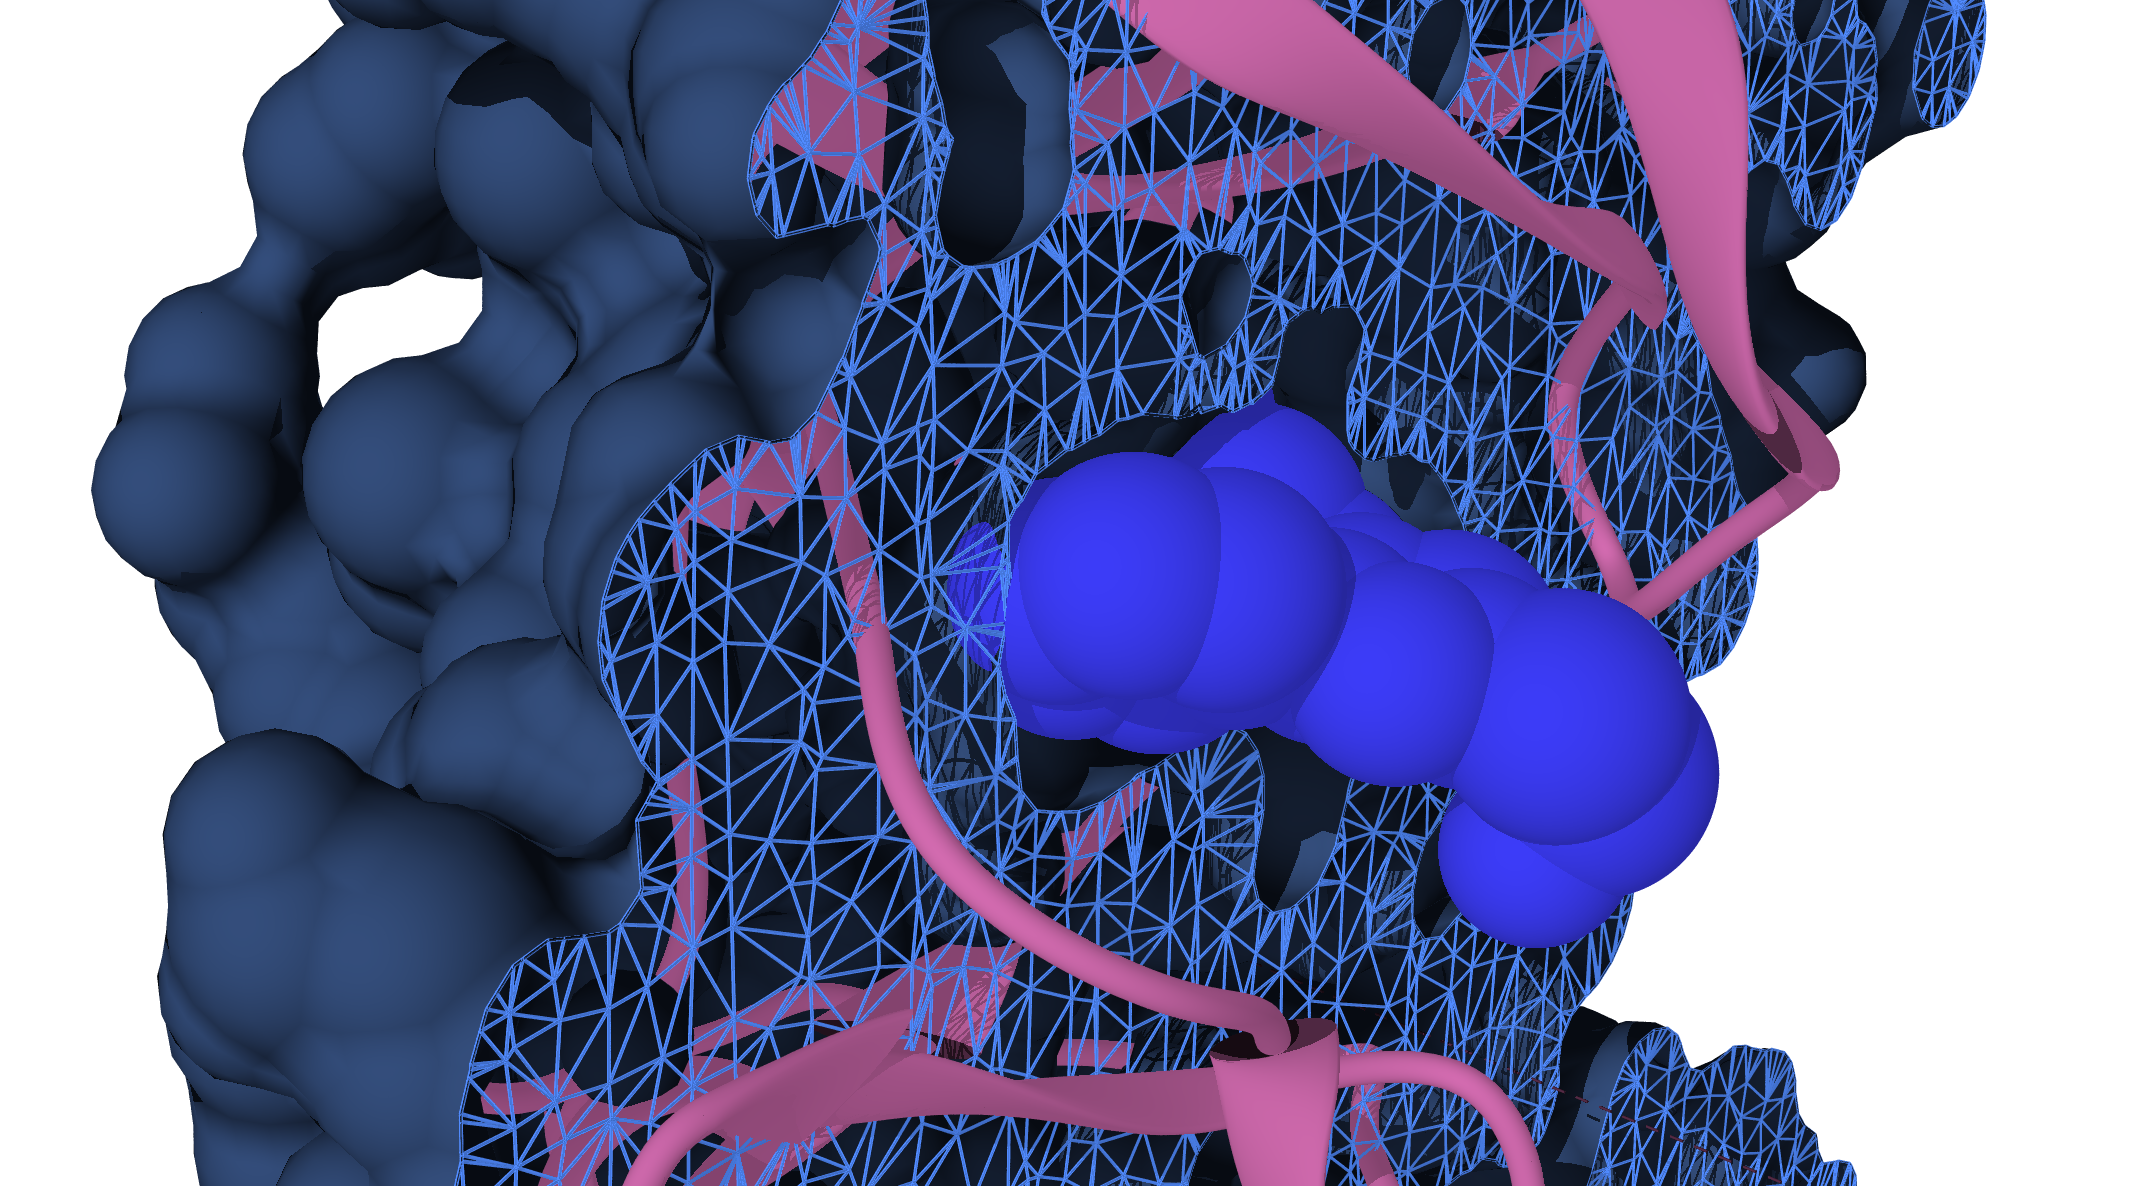
\includegraphics[width=\linewidth]{Figures/POV-render.png}
    \caption{Рендер POV-Ray}
    \label{fig:pov}
    \vspace{1em}
\end{subfigure}
\begin{subfigure}{\linewidth}
    \centering
    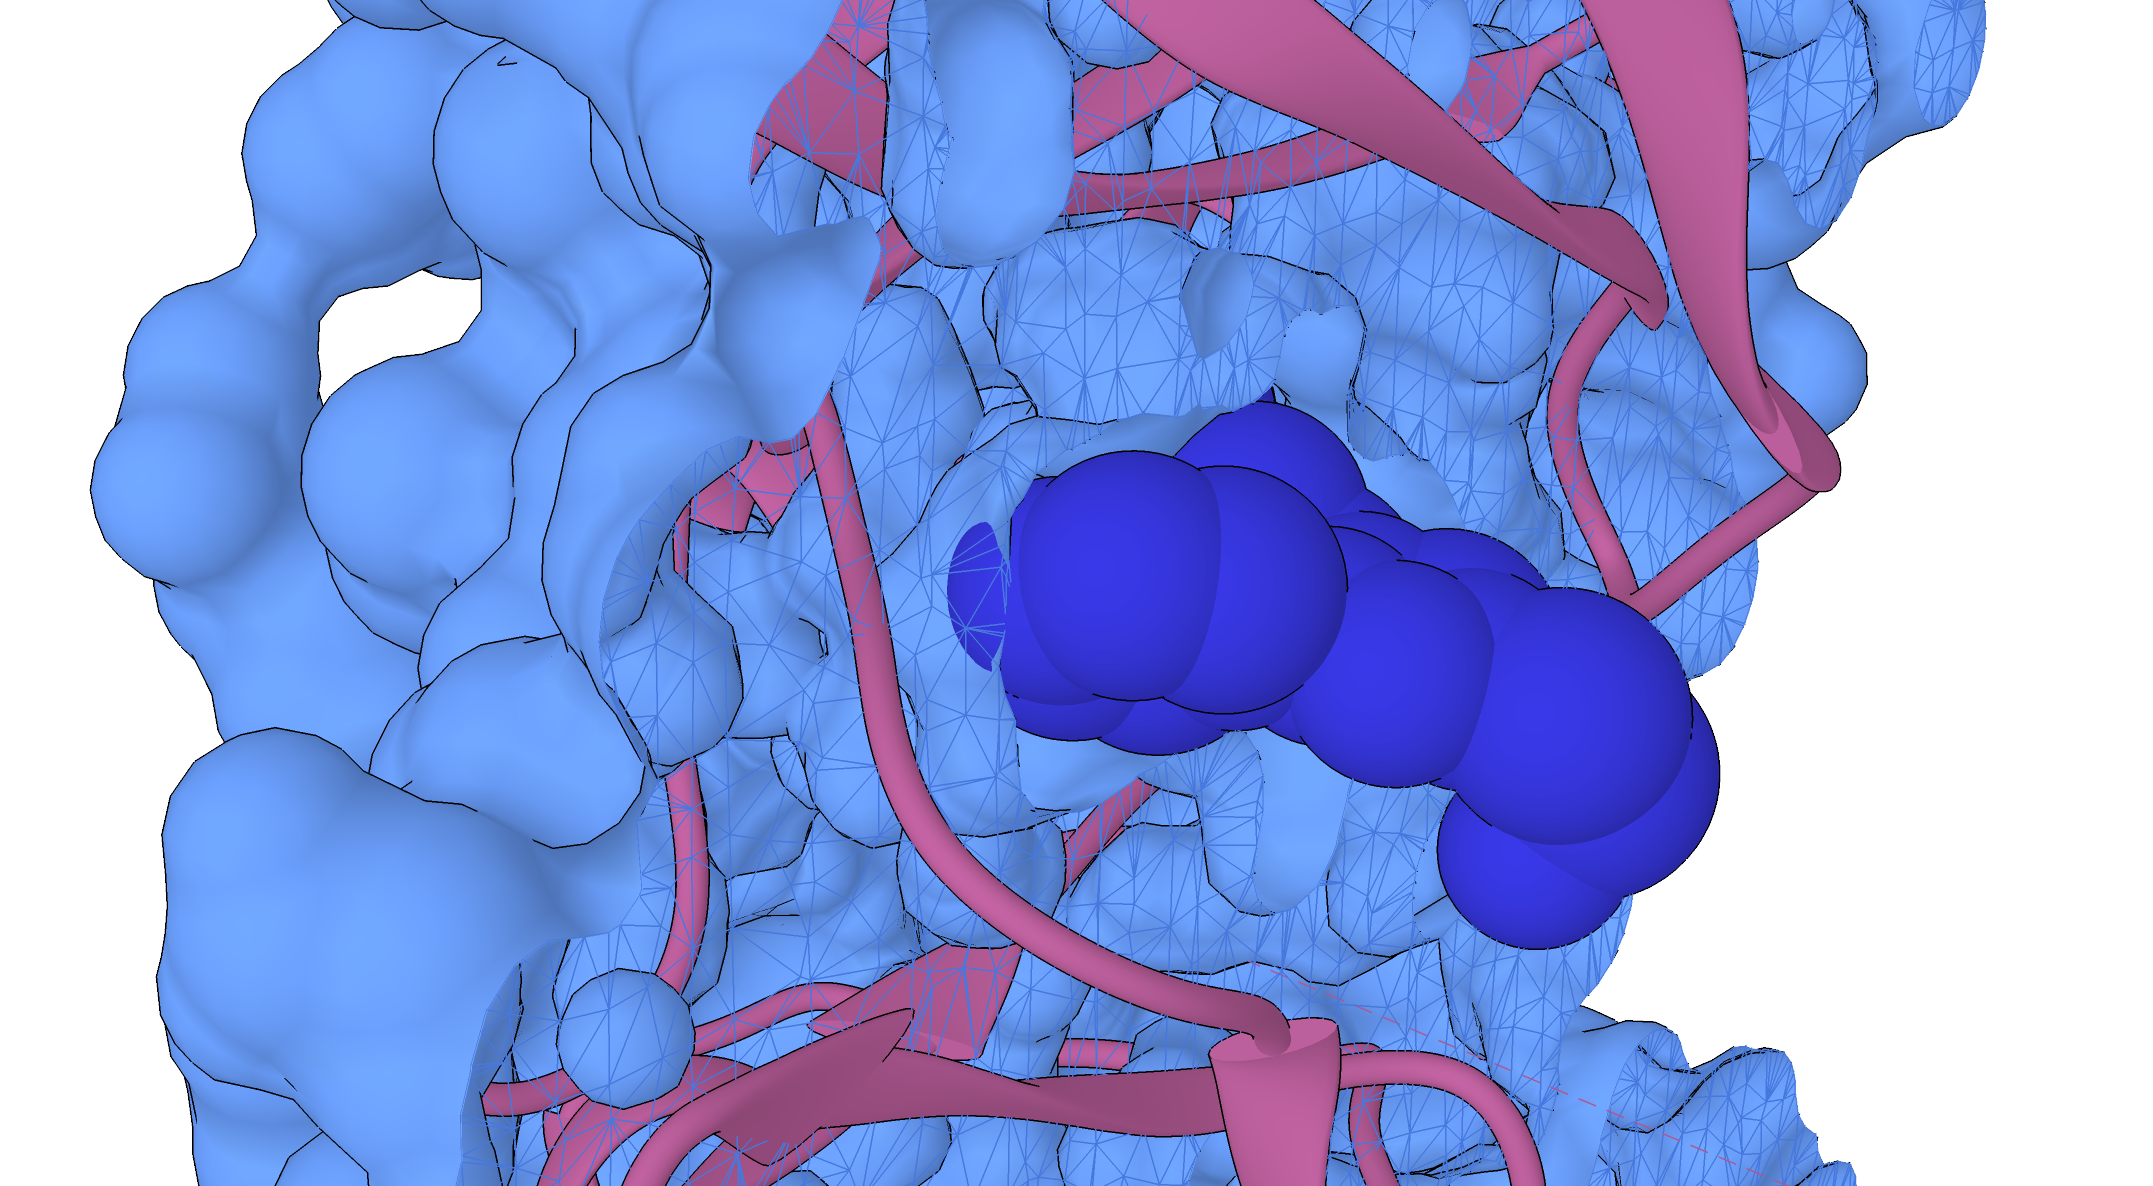
\includegraphics[width=\linewidth]{Figures/Chimera-render.png}
    \caption{Нативный рендер}
    \label{fig:chi}
\end{subfigure}
\caption{Различия между алгоритмами рендера.}
\label{fig:render}
\end{figure}\clearpage
